\documentclass[]{article}
\usepackage{lmodern}
\usepackage{amssymb,amsmath}
\usepackage{ifxetex,ifluatex}
\usepackage{fixltx2e} % provides \textsubscript
\ifnum 0\ifxetex 1\fi\ifluatex 1\fi=0 % if pdftex
  \usepackage[T1]{fontenc}
  \usepackage[utf8]{inputenc}
\else % if luatex or xelatex
  \ifxetex
    \usepackage{mathspec}
  \else
    \usepackage{fontspec}
  \fi
  \defaultfontfeatures{Ligatures=TeX,Scale=MatchLowercase}
\fi
% use upquote if available, for straight quotes in verbatim environments
\IfFileExists{upquote.sty}{\usepackage{upquote}}{}
% use microtype if available
\IfFileExists{microtype.sty}{%
\usepackage{microtype}
\UseMicrotypeSet[protrusion]{basicmath} % disable protrusion for tt fonts
}{}
\usepackage[margin=1in]{geometry}
\usepackage{hyperref}
\hypersetup{unicode=true,
            pdftitle={stats},
            pdfborder={0 0 0},
            breaklinks=true}
\urlstyle{same}  % don't use monospace font for urls
\usepackage{color}
\usepackage{fancyvrb}
\newcommand{\VerbBar}{|}
\newcommand{\VERB}{\Verb[commandchars=\\\{\}]}
\DefineVerbatimEnvironment{Highlighting}{Verbatim}{commandchars=\\\{\}}
% Add ',fontsize=\small' for more characters per line
\usepackage{framed}
\definecolor{shadecolor}{RGB}{248,248,248}
\newenvironment{Shaded}{\begin{snugshade}}{\end{snugshade}}
\newcommand{\KeywordTok}[1]{\textcolor[rgb]{0.13,0.29,0.53}{\textbf{#1}}}
\newcommand{\DataTypeTok}[1]{\textcolor[rgb]{0.13,0.29,0.53}{#1}}
\newcommand{\DecValTok}[1]{\textcolor[rgb]{0.00,0.00,0.81}{#1}}
\newcommand{\BaseNTok}[1]{\textcolor[rgb]{0.00,0.00,0.81}{#1}}
\newcommand{\FloatTok}[1]{\textcolor[rgb]{0.00,0.00,0.81}{#1}}
\newcommand{\ConstantTok}[1]{\textcolor[rgb]{0.00,0.00,0.00}{#1}}
\newcommand{\CharTok}[1]{\textcolor[rgb]{0.31,0.60,0.02}{#1}}
\newcommand{\SpecialCharTok}[1]{\textcolor[rgb]{0.00,0.00,0.00}{#1}}
\newcommand{\StringTok}[1]{\textcolor[rgb]{0.31,0.60,0.02}{#1}}
\newcommand{\VerbatimStringTok}[1]{\textcolor[rgb]{0.31,0.60,0.02}{#1}}
\newcommand{\SpecialStringTok}[1]{\textcolor[rgb]{0.31,0.60,0.02}{#1}}
\newcommand{\ImportTok}[1]{#1}
\newcommand{\CommentTok}[1]{\textcolor[rgb]{0.56,0.35,0.01}{\textit{#1}}}
\newcommand{\DocumentationTok}[1]{\textcolor[rgb]{0.56,0.35,0.01}{\textbf{\textit{#1}}}}
\newcommand{\AnnotationTok}[1]{\textcolor[rgb]{0.56,0.35,0.01}{\textbf{\textit{#1}}}}
\newcommand{\CommentVarTok}[1]{\textcolor[rgb]{0.56,0.35,0.01}{\textbf{\textit{#1}}}}
\newcommand{\OtherTok}[1]{\textcolor[rgb]{0.56,0.35,0.01}{#1}}
\newcommand{\FunctionTok}[1]{\textcolor[rgb]{0.00,0.00,0.00}{#1}}
\newcommand{\VariableTok}[1]{\textcolor[rgb]{0.00,0.00,0.00}{#1}}
\newcommand{\ControlFlowTok}[1]{\textcolor[rgb]{0.13,0.29,0.53}{\textbf{#1}}}
\newcommand{\OperatorTok}[1]{\textcolor[rgb]{0.81,0.36,0.00}{\textbf{#1}}}
\newcommand{\BuiltInTok}[1]{#1}
\newcommand{\ExtensionTok}[1]{#1}
\newcommand{\PreprocessorTok}[1]{\textcolor[rgb]{0.56,0.35,0.01}{\textit{#1}}}
\newcommand{\AttributeTok}[1]{\textcolor[rgb]{0.77,0.63,0.00}{#1}}
\newcommand{\RegionMarkerTok}[1]{#1}
\newcommand{\InformationTok}[1]{\textcolor[rgb]{0.56,0.35,0.01}{\textbf{\textit{#1}}}}
\newcommand{\WarningTok}[1]{\textcolor[rgb]{0.56,0.35,0.01}{\textbf{\textit{#1}}}}
\newcommand{\AlertTok}[1]{\textcolor[rgb]{0.94,0.16,0.16}{#1}}
\newcommand{\ErrorTok}[1]{\textcolor[rgb]{0.64,0.00,0.00}{\textbf{#1}}}
\newcommand{\NormalTok}[1]{#1}
\usepackage{graphicx,grffile}
\makeatletter
\def\maxwidth{\ifdim\Gin@nat@width>\linewidth\linewidth\else\Gin@nat@width\fi}
\def\maxheight{\ifdim\Gin@nat@height>\textheight\textheight\else\Gin@nat@height\fi}
\makeatother
% Scale images if necessary, so that they will not overflow the page
% margins by default, and it is still possible to overwrite the defaults
% using explicit options in \includegraphics[width, height, ...]{}
\setkeys{Gin}{width=\maxwidth,height=\maxheight,keepaspectratio}
\IfFileExists{parskip.sty}{%
\usepackage{parskip}
}{% else
\setlength{\parindent}{0pt}
\setlength{\parskip}{6pt plus 2pt minus 1pt}
}
\setlength{\emergencystretch}{3em}  % prevent overfull lines
\providecommand{\tightlist}{%
  \setlength{\itemsep}{0pt}\setlength{\parskip}{0pt}}
\setcounter{secnumdepth}{0}
% Redefines (sub)paragraphs to behave more like sections
\ifx\paragraph\undefined\else
\let\oldparagraph\paragraph
\renewcommand{\paragraph}[1]{\oldparagraph{#1}\mbox{}}
\fi
\ifx\subparagraph\undefined\else
\let\oldsubparagraph\subparagraph
\renewcommand{\subparagraph}[1]{\oldsubparagraph{#1}\mbox{}}
\fi

%%% Use protect on footnotes to avoid problems with footnotes in titles
\let\rmarkdownfootnote\footnote%
\def\footnote{\protect\rmarkdownfootnote}

%%% Change title format to be more compact
\usepackage{titling}

% Create subtitle command for use in maketitle
\newcommand{\subtitle}[1]{
  \posttitle{
    \begin{center}\large#1\end{center}
    }
}

\setlength{\droptitle}{-2em}
  \title{stats}
  \pretitle{\vspace{\droptitle}\centering\huge}
  \posttitle{\par}
  \author{}
  \preauthor{}\postauthor{}
  \date{}
  \predate{}\postdate{}

\usepackage{amsmath}
\usepackage{mathtools}
\usepackage{float}
\usepackage{xcolor,pifont}
\newcommand{\cmark}{\Large\textcolor{green}{\ding{52}}}
\newcommand{\xmark}{\Large\textcolor{red}{\ding{55}}}

\begin{document}
\maketitle

\begin{Shaded}
\begin{Highlighting}[]
\KeywordTok{require}\NormalTok{(dplyr)}
\end{Highlighting}
\end{Shaded}

\begin{verbatim}
## Loading required package: dplyr
\end{verbatim}

\begin{verbatim}
## 
## Attaching package: 'dplyr'
\end{verbatim}

\begin{verbatim}
## The following objects are masked from 'package:stats':
## 
##     filter, lag
\end{verbatim}

\begin{verbatim}
## The following objects are masked from 'package:base':
## 
##     intersect, setdiff, setequal, union
\end{verbatim}

\begin{Shaded}
\begin{Highlighting}[]
\KeywordTok{require}\NormalTok{(tidyr)}
\end{Highlighting}
\end{Shaded}

\begin{verbatim}
## Loading required package: tidyr
\end{verbatim}

\begin{Shaded}
\begin{Highlighting}[]
\KeywordTok{require}\NormalTok{(knitr)}
\end{Highlighting}
\end{Shaded}

\begin{verbatim}
## Loading required package: knitr
\end{verbatim}

\begin{Shaded}
\begin{Highlighting}[]
\KeywordTok{require}\NormalTok{(ggplot2)}
\end{Highlighting}
\end{Shaded}

\begin{verbatim}
## Loading required package: ggplot2
\end{verbatim}

\begin{Shaded}
\begin{Highlighting}[]
\KeywordTok{require}\NormalTok{(maps)}
\end{Highlighting}
\end{Shaded}

\begin{verbatim}
## Loading required package: maps
\end{verbatim}

\begin{Shaded}
\begin{Highlighting}[]
\KeywordTok{require}\NormalTok{(RColorBrewer)}
\end{Highlighting}
\end{Shaded}

\begin{verbatim}
## Loading required package: RColorBrewer
\end{verbatim}

\begin{Shaded}
\begin{Highlighting}[]
\KeywordTok{require}\NormalTok{(summarytools)}
\end{Highlighting}
\end{Shaded}

\begin{verbatim}
## Loading required package: summarytools
\end{verbatim}

\begin{verbatim}
## Loading required package: htmltools
\end{verbatim}

\begin{Shaded}
\begin{Highlighting}[]
\KeywordTok{sessionInfo}\NormalTok{()}
\end{Highlighting}
\end{Shaded}

\begin{verbatim}
## R version 3.3.2 (2016-10-31)
## Platform: x86_64-w64-mingw32/x64 (64-bit)
## Running under: Windows 10 x64 (build 16299)
## 
## locale:
## [1] LC_COLLATE=English_United States.1252 
## [2] LC_CTYPE=English_United States.1252   
## [3] LC_MONETARY=English_United States.1252
## [4] LC_NUMERIC=C                          
## [5] LC_TIME=English_United States.1252    
## 
## attached base packages:
## [1] stats     graphics  grDevices utils     datasets  methods   base     
## 
## other attached packages:
##  [1] summarytools_0.4     htmltools_0.3.5      RColorBrewer_1.1-2  
##  [4] maps_3.1.1           ggplot2_2.1.0        knitr_1.20          
##  [7] tidyr_0.6.0          dplyr_0.5.0          RevoUtilsMath_10.0.0
## [10] RevoUtils_10.0.2     RevoMods_10.0.0      MicrosoftML_1.0.0   
## [13] mrsdeploy_1.0        RevoScaleR_9.0.1     lattice_0.20-34     
## [16] rpart_4.1-10        
## 
## loaded via a namespace (and not attached):
##  [1] Rcpp_0.12.9            plyr_1.8.4             iterators_1.0.8       
##  [4] tools_3.3.2            digest_0.6.12          jsonlite_1.1          
##  [7] evaluate_0.10          tibble_1.2             gtable_0.2.0          
## [10] foreach_1.4.3          DBI_0.5-1              CompatibilityAPI_1.1.0
## [13] curl_2.2               yaml_2.1.14            stringr_1.3.1         
## [16] rprojroot_1.3-2        grid_3.3.2             R6_2.2.0              
## [19] rmarkdown_1.9          magrittr_1.5           backports_1.1.2       
## [22] scales_0.4.1           codetools_0.2-15       assertthat_0.1        
## [25] colorspace_1.3-2       stringi_1.1.7          munsell_0.4.3
\end{verbatim}

\begin{Shaded}
\begin{Highlighting}[]
\NormalTok{beer_data <-}\StringTok{ }\KeywordTok{read.csv}\NormalTok{(}\StringTok{"../data/Beers.csv"}\NormalTok{, }\DataTypeTok{header=}\OtherTok{TRUE}\NormalTok{)}


\KeywordTok{head}\NormalTok{(beer_data)}
\end{Highlighting}
\end{Shaded}

\begin{verbatim}
##                  Name Beer_ID   ABV IBU Brewery_id
## 1            Pub Beer    1436 0.050  NA        409
## 2         Devil's Cup    2265 0.066  NA        178
## 3 Rise of the Phoenix    2264 0.071  NA        178
## 4            Sinister    2263 0.090  NA        178
## 5       Sex and Candy    2262 0.075  NA        178
## 6        Black Exodus    2261 0.077  NA        178
##                            Style Ounces
## 1            American Pale Lager     12
## 2        American Pale Ale (APA)     12
## 3                   American IPA     12
## 4 American Double / Imperial IPA     12
## 5                   American IPA     12
## 6                  Oatmeal Stout     12
\end{verbatim}

\begin{Shaded}
\begin{Highlighting}[]
\CommentTok{#beer_data$Brewery_id[(beer_data$Brewery_id %in% breweries_sk$Brew_ID)]  <- breweries_sk$Brew_SK # update brewery_ids from brewery_sk data}


\NormalTok{beer_clean <-}\StringTok{ }\KeywordTok{distinct}\NormalTok{(beer_data) }\OperatorTok\StringTok{ }\KeywordTok{rename}\NormalTok{(}\DataTypeTok{Brew_ID =}\NormalTok{ Brewery_id, }\DataTypeTok{Beer_Name =}\NormalTok{ Name) }

\NormalTok{notnull <-}\StringTok{ }\NormalTok{beer_data }\OperatorTok\StringTok{ }\KeywordTok{filter}\NormalTok{(}\KeywordTok{is.na}\NormalTok{(IBU)) }\OperatorTok\StringTok{ }\KeywordTok{distinct}\NormalTok{(Style)}


\NormalTok{isnull <-}\StringTok{ }\NormalTok{beer_data }\OperatorTok\StringTok{ }\KeywordTok{filter}\NormalTok{(}\OperatorTok{!}\KeywordTok{is.na}\NormalTok{(IBU)) }\OperatorTok\StringTok{ }\KeywordTok{distinct}\NormalTok{(Style, IBU, ABV, Ounces) }\OperatorTok\StringTok{ }\KeywordTok{arrange}\NormalTok{(Style)}


\CommentTok{#A distinct list of beer styles. A distinct beer style is noted as having a unique style name, IBU, ABV, and Ounces values.}
\NormalTok{styles <-}\StringTok{ }\NormalTok{notnull }\OperatorTok\StringTok{ }
\StringTok{          }\KeywordTok{full_join}\NormalTok{(isnull, }\DataTypeTok{by =} \StringTok{"Style"}\NormalTok{) }\OperatorTok\StringTok{ }\KeywordTok{arrange}\NormalTok{(Style) }\CommentTok{#%>%}
          \CommentTok{#mutate_each(funs(as.character), Style)}

\NormalTok{styles <-}\StringTok{ }\NormalTok{styles }\OperatorTok\StringTok{ }\KeywordTok{na.omit}\NormalTok{(IBU, ABV) }\CommentTok{#omit any record with missing ABV or IBU}

\NormalTok{ss <-}\StringTok{ }\KeywordTok{sample_n}\NormalTok{(styles, }\DataTypeTok{size =} \DecValTok{30}\NormalTok{) }\CommentTok{#sample data frame rows so IBU and ABV remain paired}
\end{Highlighting}
\end{Shaded}

\begin{Shaded}
\begin{Highlighting}[]
\NormalTok{lm_eqn =}\StringTok{ }\ControlFlowTok{function}\NormalTok{(m) \{}

\NormalTok{  l <-}\StringTok{ }\KeywordTok{list}\NormalTok{(}\DataTypeTok{a =} \KeywordTok{format}\NormalTok{(}\KeywordTok{coef}\NormalTok{(m)[}\DecValTok{1}\NormalTok{], }\DataTypeTok{digits =} \DecValTok{2}\NormalTok{),}
      \DataTypeTok{b =} \KeywordTok{format}\NormalTok{(}\KeywordTok{abs}\NormalTok{(}\KeywordTok{coef}\NormalTok{(m)[}\DecValTok{2}\NormalTok{]), }\DataTypeTok{digits =} \DecValTok{2}\NormalTok{),}
      \DataTypeTok{r2 =} \KeywordTok{format}\NormalTok{(}\KeywordTok{summary}\NormalTok{(m)}\OperatorTok{$}\NormalTok{r.squared, }\DataTypeTok{digits =} \DecValTok{3}\NormalTok{));}

  \ControlFlowTok{if}\NormalTok{ (}\KeywordTok{coef}\NormalTok{(m)[}\DecValTok{2}\NormalTok{] }\OperatorTok{>=}\StringTok{ }\DecValTok{0}\NormalTok{)  \{}
\NormalTok{    eq <-}\StringTok{ }\KeywordTok{substitute}\NormalTok{(}\KeywordTok{italic}\NormalTok{(y) }\OperatorTok{==}\StringTok{ }\NormalTok{a }\OperatorTok{+}\StringTok{ }\NormalTok{b }\OperatorTok\StringTok{ }\KeywordTok{italic}\NormalTok{(x)}\OperatorTok{*}\StringTok{","}\OperatorTok{~}\ErrorTok{~}\KeywordTok{italic}\NormalTok{(r)}\OperatorTok{^}\DecValTok{2}\OperatorTok{~}\StringTok{"="}\OperatorTok{~}\NormalTok{r2,l)}
\NormalTok{  \} }\ControlFlowTok{else}\NormalTok{ \{}
\NormalTok{    eq <-}\StringTok{ }\KeywordTok{substitute}\NormalTok{(}\KeywordTok{italic}\NormalTok{(y) }\OperatorTok{==}\StringTok{ }\NormalTok{a }\OperatorTok{-}\StringTok{ }\NormalTok{b }\OperatorTok\StringTok{ }\KeywordTok{italic}\NormalTok{(x)}\OperatorTok{*}\StringTok{","}\OperatorTok{~}\ErrorTok{~}\KeywordTok{italic}\NormalTok{(r)}\OperatorTok{^}\DecValTok{2}\OperatorTok{~}\StringTok{"="}\OperatorTok{~}\NormalTok{r2,l)    }
\NormalTok{  \}}

  \KeywordTok{as.character}\NormalTok{(}\KeywordTok{as.expression}\NormalTok{(eq));                 }
\NormalTok{\}}
\KeywordTok{ggplot}\NormalTok{(ss, }\KeywordTok{aes}\NormalTok{(}\DataTypeTok{x=}\NormalTok{ABV, }\DataTypeTok{y=}\NormalTok{IBU)) }\OperatorTok{+}
\StringTok{  }\KeywordTok{geom_point}\NormalTok{() }\OperatorTok{+}
\StringTok{  }\KeywordTok{geom_smooth}\NormalTok{(}\DataTypeTok{method =} \StringTok{"lm"}\NormalTok{) }\OperatorTok{+}
\StringTok{  }\KeywordTok{geom_text}\NormalTok{(}\KeywordTok{aes}\NormalTok{(}\DataTypeTok{x =}\NormalTok{ .}\DecValTok{06}\NormalTok{, }\DataTypeTok{y =} \DecValTok{100}\NormalTok{, }\DataTypeTok{label =} \KeywordTok{lm_eqn}\NormalTok{(}\KeywordTok{lm}\NormalTok{(ABV }\OperatorTok{~}\StringTok{ }\NormalTok{IBU ,ss))), }\DataTypeTok{parse =} \OtherTok{TRUE}\NormalTok{, }\DataTypeTok{color =} \StringTok{"red"}\NormalTok{)}
\end{Highlighting}
\end{Shaded}

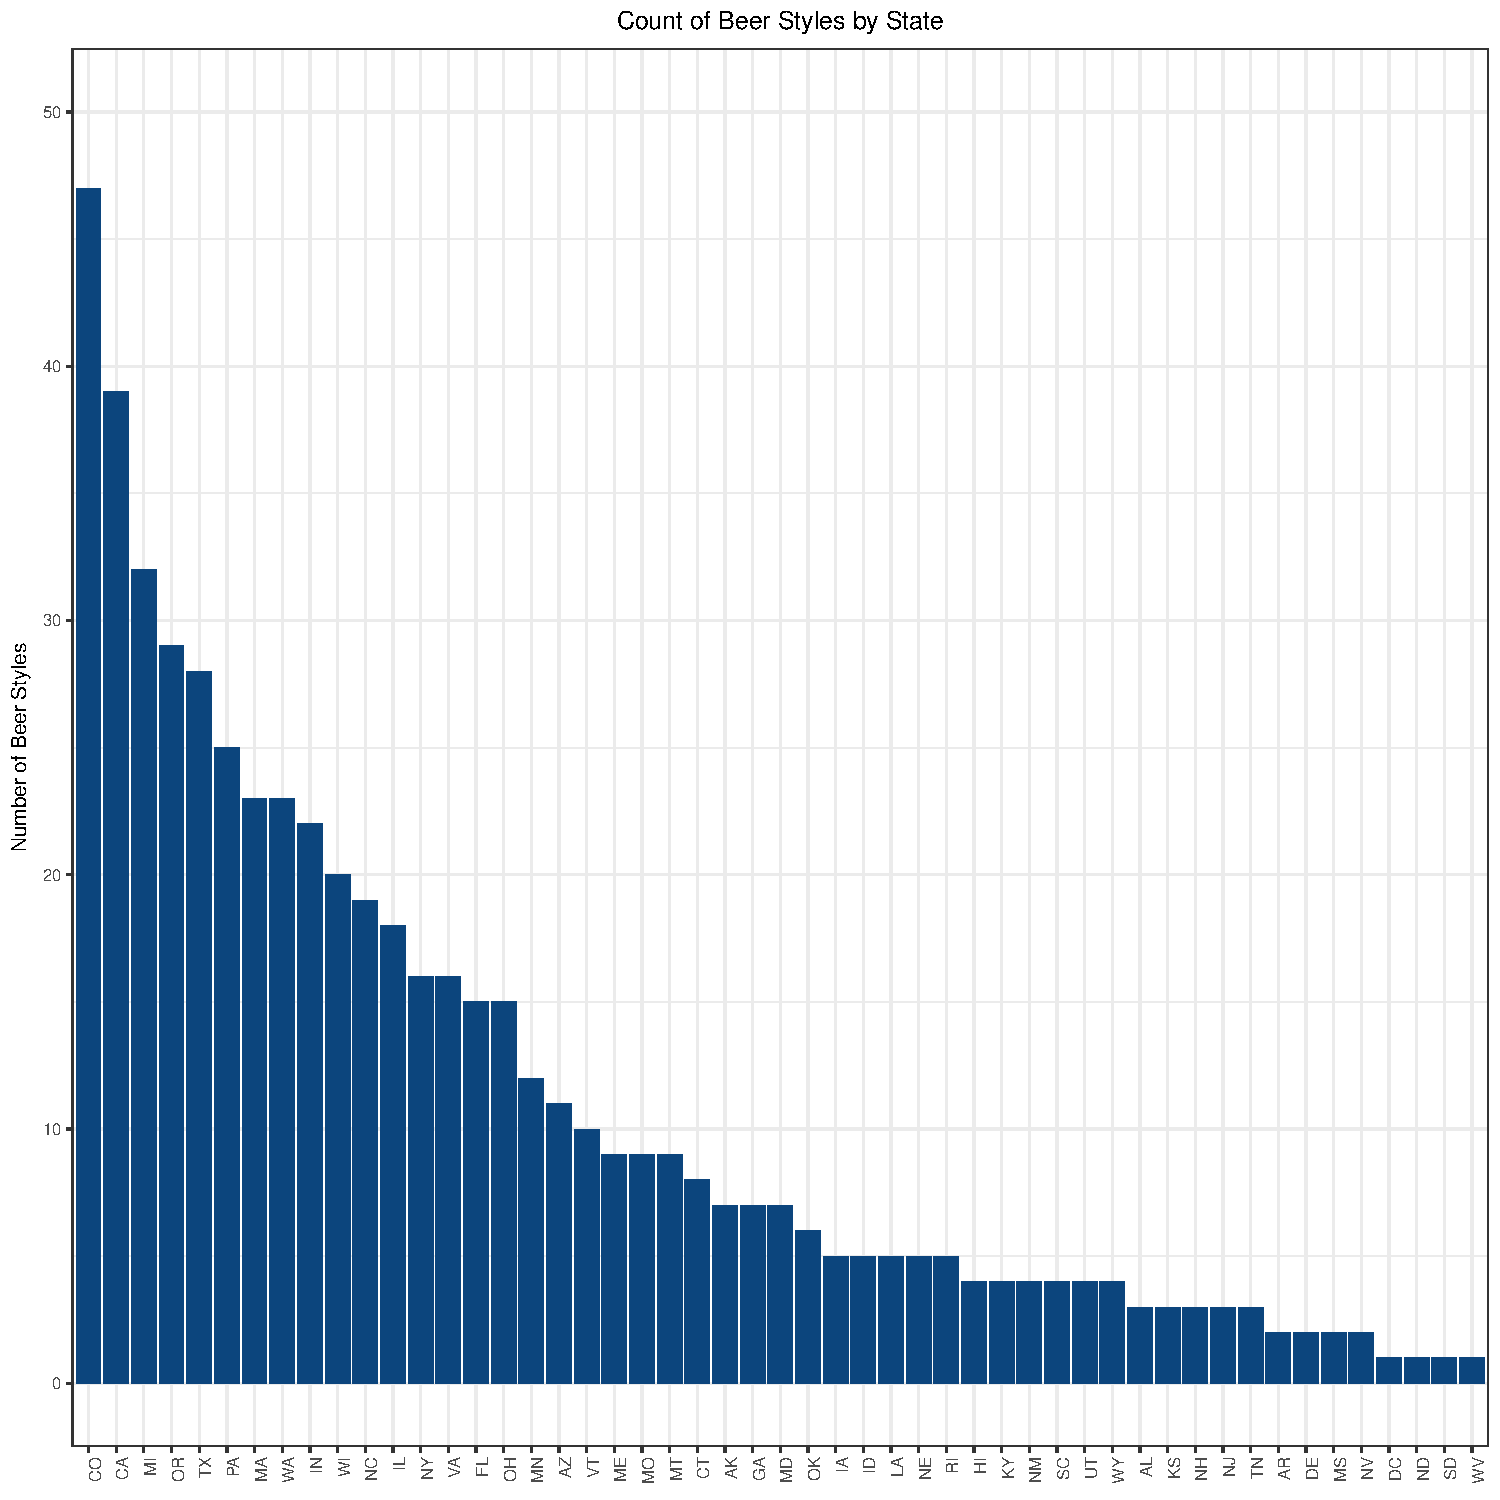
\includegraphics{stats_files/figure-latex/unnamed-chunk-3-1.pdf}

\begin{Shaded}
\begin{Highlighting}[]
\KeywordTok{ggplot}\NormalTok{(styles, }\KeywordTok{aes}\NormalTok{(}\DataTypeTok{x=}\NormalTok{ABV, }\DataTypeTok{y=}\NormalTok{IBU)) }\OperatorTok{+}
\StringTok{  }\KeywordTok{geom_point}\NormalTok{(}\KeywordTok{aes}\NormalTok{(}\DataTypeTok{colour=}\KeywordTok{as.factor}\NormalTok{(Ounces))) }\OperatorTok{+}
\StringTok{  }\KeywordTok{scale_colour_brewer}\NormalTok{() }\OperatorTok{+}
\StringTok{  }\KeywordTok{geom_smooth}\NormalTok{(}\DataTypeTok{method =} \StringTok{"lm"}\NormalTok{) }\OperatorTok{+}
\StringTok{  }\KeywordTok{theme}\NormalTok{(}\DataTypeTok{legend.position=}\StringTok{"none"}\NormalTok{)}
\end{Highlighting}
\end{Shaded}

\includegraphics{stats_files/figure-latex/unnamed-chunk-3-2.pdf}

\begin{Shaded}
\begin{Highlighting}[]
  \CommentTok{#geom_text(aes(x = .06, y = 100, label = lm_eqn(lm(ABV ~ IBU ,styles))), parse = TRUE, color = "red")}
\end{Highlighting}
\end{Shaded}

\section{Check for Outliers in IBU}\label{check-for-outliers-in-ibu}

\begin{Shaded}
\begin{Highlighting}[]
\NormalTok{ibu_outliers <-}\StringTok{ }\KeywordTok{boxplot}\NormalTok{(styles}\OperatorTok{$}\NormalTok{IBU, }\DataTypeTok{plot =} \OtherTok{FALSE}\NormalTok{)[[}\StringTok{"out"}\NormalTok{]]}

\KeywordTok{ggplot}\NormalTok{((styles }\OperatorTok\StringTok{ }\KeywordTok{drop_na}\NormalTok{(IBU)), }\KeywordTok{aes}\NormalTok{(}\DataTypeTok{x=}\StringTok{""}\NormalTok{, }\DataTypeTok{y=}\NormalTok{IBU)) }\OperatorTok{+}
\StringTok{      }\KeywordTok{geom_point}\NormalTok{(}\KeywordTok{aes}\NormalTok{(}\DataTypeTok{fill =} \KeywordTok{ifelse}\NormalTok{((IBU }\OperatorTok\StringTok{ }\NormalTok{ibu_outliers),}\StringTok{"Outlier"}\NormalTok{,}\StringTok{"Valid"}\NormalTok{)), }\DataTypeTok{size =} \DecValTok{5}\NormalTok{, }\DataTypeTok{shape =} \DecValTok{21}\NormalTok{, }\DataTypeTok{position =} \KeywordTok{position_jitter}\NormalTok{())}\OperatorTok{+}
\StringTok{      }\KeywordTok{stat_boxplot}\NormalTok{(}\DataTypeTok{geom =}\StringTok{'errorbar'}\NormalTok{) }\OperatorTok{+}
\StringTok{      }\KeywordTok{geom_boxplot}\NormalTok{(}\DataTypeTok{alpha=}\NormalTok{.}\DecValTok{5}\NormalTok{, }\DataTypeTok{outlier.shape =} \OtherTok{NA}\NormalTok{) }\OperatorTok{+}\CommentTok{#, outlier.colour = "red") +}
\StringTok{      }\KeywordTok{stat_summary}\NormalTok{(}\DataTypeTok{fun.y=}\NormalTok{mean, }\DataTypeTok{geom=}\StringTok{"point"}\NormalTok{, }\DataTypeTok{shape=}\DecValTok{5}\NormalTok{, }\DataTypeTok{size=}\DecValTok{4}\NormalTok{) }\OperatorTok{+}
\StringTok{      }\KeywordTok{coord_flip}\NormalTok{()}
\end{Highlighting}
\end{Shaded}

\includegraphics{stats_files/figure-latex/unnamed-chunk-4-1.pdf}

\begin{Shaded}
\begin{Highlighting}[]
      \CommentTok{#geom_text(aes(label=ifelse((x>4*IQR(x)|y>4*IQR(y)),label,"")), hjust=1.1)}



\NormalTok{ibu_outliers}
\end{Highlighting}
\end{Shaded}

\begin{verbatim}
## [1] 138 130 126 135
\end{verbatim}

\section{Check for Outliers in ABV}\label{check-for-outliers-in-abv}

\begin{Shaded}
\begin{Highlighting}[]
\NormalTok{abv_outliers <-}\StringTok{ }\KeywordTok{boxplot}\NormalTok{(styles}\OperatorTok{$}\NormalTok{ABV, }\DataTypeTok{plot =} \OtherTok{FALSE}\NormalTok{)[[}\StringTok{"out"}\NormalTok{]]}

\NormalTok{abv_outliers}
\end{Highlighting}
\end{Shaded}

\begin{verbatim}
##  [1] 0.099 0.099 0.099 0.099 0.099 0.097 0.098 0.099 0.096 0.099 0.099
## [12] 0.099 0.097 0.099 0.099 0.099 0.099 0.100 0.099 0.099 0.125 0.099
## [23] 0.099 0.099 0.099 0.120 0.099
\end{verbatim}

\begin{Shaded}
\begin{Highlighting}[]
\KeywordTok{ggplot}\NormalTok{((styles }\OperatorTok\StringTok{ }\KeywordTok{drop_na}\NormalTok{(ABV)), }\KeywordTok{aes}\NormalTok{(}\DataTypeTok{x=}\StringTok{""}\NormalTok{, }\DataTypeTok{y=}\NormalTok{ABV)) }\OperatorTok{+}
\StringTok{      }\CommentTok{#geom_point(aes(fill = ifelse((ABV>3.29*IQR(ABV)),"Outlier","Valid")), size = 5, shape = 21, position = position_jitter())+#= position_jitterdodge()) +}
\StringTok{      }\KeywordTok{geom_point}\NormalTok{(}\KeywordTok{aes}\NormalTok{(}\DataTypeTok{fill =} \KeywordTok{ifelse}\NormalTok{((ABV }\OperatorTok\StringTok{ }\NormalTok{abv_outliers),}\StringTok{"Outlier"}\NormalTok{,}\StringTok{"Valid"}\NormalTok{)), }\DataTypeTok{size =} \DecValTok{5}\NormalTok{, }\DataTypeTok{shape =} \DecValTok{21}\NormalTok{, }\DataTypeTok{position =} \KeywordTok{position_jitter}\NormalTok{())}\OperatorTok{+}
\StringTok{      }\KeywordTok{stat_boxplot}\NormalTok{(}\DataTypeTok{geom =}\StringTok{'errorbar'}\NormalTok{) }\OperatorTok{+}
\StringTok{      }\KeywordTok{geom_boxplot}\NormalTok{(}\DataTypeTok{alpha=}\NormalTok{.}\DecValTok{5}\NormalTok{, }\DataTypeTok{outlier.shape =} \OtherTok{NA}\NormalTok{) }\OperatorTok{+}\CommentTok{#, outlier.colour = "red") +}
\StringTok{      }\KeywordTok{stat_summary}\NormalTok{(}\DataTypeTok{fun.y=}\NormalTok{mean, }\DataTypeTok{geom=}\StringTok{"point"}\NormalTok{, }\DataTypeTok{shape=}\DecValTok{5}\NormalTok{, }\DataTypeTok{size=}\DecValTok{4}\NormalTok{) }\OperatorTok{+}\StringTok{ }
\StringTok{      }\KeywordTok{coord_flip}\NormalTok{()}
\end{Highlighting}
\end{Shaded}

\includegraphics{stats_files/figure-latex/unnamed-chunk-5-1.pdf}

\begin{Shaded}
\begin{Highlighting}[]
      \CommentTok{#geom_text(aes(label=ifelse((x>4*IQR(x)|y>4*IQR(y)),label,"")), hjust=1.1)}

\CommentTok{#boxplot(styles$ABV, plot = TRUE)}
\end{Highlighting}
\end{Shaded}

\section{check normality of full dataset and
sample}\label{check-normality-of-full-dataset-and-sample}

\begin{Shaded}
\begin{Highlighting}[]
\CommentTok{#full dataaset}
\KeywordTok{ggplot}\NormalTok{(styles) }\OperatorTok{+}
\StringTok{    }\KeywordTok{geom_histogram}\NormalTok{(}\KeywordTok{aes}\NormalTok{(}\DataTypeTok{x=}\NormalTok{IBU)) }\OperatorTok{+}
\StringTok{    }\KeywordTok{theme}\NormalTok{(}\DataTypeTok{text =} \KeywordTok{element_text}\NormalTok{(}\DataTypeTok{size=}\DecValTok{10}\NormalTok{),}
        \DataTypeTok{axis.text.x =} \KeywordTok{element_text}\NormalTok{(}\DataTypeTok{angle=}\DecValTok{90}\NormalTok{, }\DataTypeTok{hjust=}\DecValTok{1}\NormalTok{)) }
\end{Highlighting}
\end{Shaded}

\begin{verbatim}
## `stat_bin()` using `bins = 30`. Pick better value with `binwidth`.
\end{verbatim}

\includegraphics{stats_files/figure-latex/unnamed-chunk-6-1.pdf}

\begin{Shaded}
\begin{Highlighting}[]
\KeywordTok{ggplot}\NormalTok{(styles) }\OperatorTok{+}
\StringTok{    }\KeywordTok{geom_histogram}\NormalTok{(}\KeywordTok{aes}\NormalTok{(}\DataTypeTok{x=}\NormalTok{ABV)) }\OperatorTok{+}
\StringTok{    }\KeywordTok{theme}\NormalTok{(}\DataTypeTok{text =} \KeywordTok{element_text}\NormalTok{(}\DataTypeTok{size=}\DecValTok{10}\NormalTok{),}
        \DataTypeTok{axis.text.x =} \KeywordTok{element_text}\NormalTok{(}\DataTypeTok{angle=}\DecValTok{90}\NormalTok{, }\DataTypeTok{hjust=}\DecValTok{1}\NormalTok{)) }
\end{Highlighting}
\end{Shaded}

\begin{verbatim}
## `stat_bin()` using `bins = 30`. Pick better value with `binwidth`.
\end{verbatim}

\includegraphics{stats_files/figure-latex/unnamed-chunk-6-2.pdf}

\begin{Shaded}
\begin{Highlighting}[]
\CommentTok{# #sample}
\CommentTok{# ggplot(ss) +}
\CommentTok{#     geom_histogram(aes(x=IBU)) +}
\CommentTok{#     theme(text = element_text(size=10),}
\CommentTok{#         axis.text.x = element_text(angle=90, hjust=1)) }
\CommentTok{# }
\CommentTok{# ggplot(ss) +}
\CommentTok{#     geom_histogram(aes(x=ABV)) +}
\CommentTok{#     theme(text = element_text(size=10),}
\CommentTok{#         axis.text.x = element_text(angle=90, hjust=1)) }
\CommentTok{# }
\CommentTok{# }
\end{Highlighting}
\end{Shaded}

\section{Check normality of log
sample}\label{check-normality-of-log-sample}

\begin{Shaded}
\begin{Highlighting}[]
\NormalTok{styles}\OperatorTok{$}\NormalTok{IBU_log <-}\StringTok{ }\KeywordTok{log}\NormalTok{(styles}\OperatorTok{$}\NormalTok{IBU)}
\NormalTok{styles}\OperatorTok{$}\NormalTok{ABV_log <-}\StringTok{ }\KeywordTok{log}\NormalTok{(styles}\OperatorTok{$}\NormalTok{ABV)}

\KeywordTok{ggplot}\NormalTok{(styles) }\OperatorTok{+}
\StringTok{    }\KeywordTok{geom_histogram}\NormalTok{(}\KeywordTok{aes}\NormalTok{(}\DataTypeTok{x=}\NormalTok{IBU_log)) }\OperatorTok{+}
\StringTok{    }\KeywordTok{theme}\NormalTok{(}\DataTypeTok{text =} \KeywordTok{element_text}\NormalTok{(}\DataTypeTok{size=}\DecValTok{10}\NormalTok{),}
        \DataTypeTok{axis.text.x =} \KeywordTok{element_text}\NormalTok{(}\DataTypeTok{angle=}\DecValTok{90}\NormalTok{, }\DataTypeTok{hjust=}\DecValTok{1}\NormalTok{)) }
\end{Highlighting}
\end{Shaded}

\begin{verbatim}
## `stat_bin()` using `bins = 30`. Pick better value with `binwidth`.
\end{verbatim}

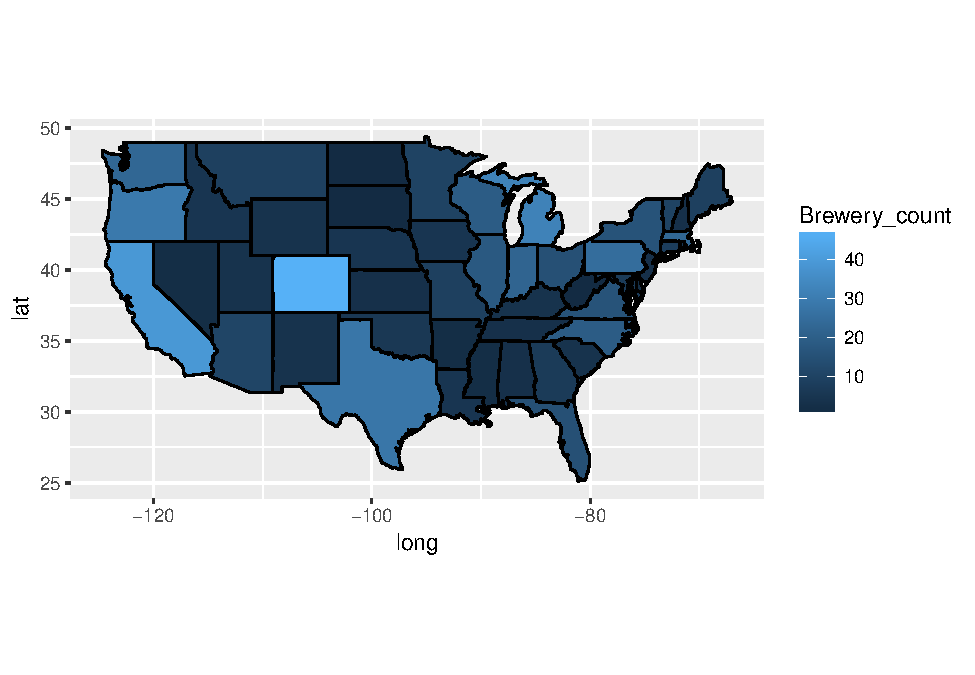
\includegraphics{stats_files/figure-latex/unnamed-chunk-7-1.pdf}

\begin{Shaded}
\begin{Highlighting}[]
\KeywordTok{ggplot}\NormalTok{(styles) }\OperatorTok{+}
\StringTok{    }\KeywordTok{geom_histogram}\NormalTok{(}\KeywordTok{aes}\NormalTok{(}\DataTypeTok{x=}\NormalTok{ABV_log)) }\OperatorTok{+}
\StringTok{    }\KeywordTok{geom_density}\NormalTok{() }\OperatorTok{+}
\StringTok{    }\KeywordTok{theme}\NormalTok{(}\DataTypeTok{text =} \KeywordTok{element_text}\NormalTok{(}\DataTypeTok{size=}\DecValTok{10}\NormalTok{),}
        \DataTypeTok{axis.text.x =} \KeywordTok{element_text}\NormalTok{(}\DataTypeTok{angle=}\DecValTok{90}\NormalTok{, }\DataTypeTok{hjust=}\DecValTok{1}\NormalTok{)) }
\end{Highlighting}
\end{Shaded}

\begin{verbatim}
## `stat_bin()` using `bins = 30`. Pick better value with `binwidth`.
\end{verbatim}

\begin{verbatim}
## Warning in max(w): no non-missing arguments to max; returning -Inf
\end{verbatim}

\begin{verbatim}
## Warning: Computation failed in `stat_density()`:
## arguments imply differing number of rows: 0, 1
\end{verbatim}

\includegraphics{stats_files/figure-latex/unnamed-chunk-7-2.pdf}

\begin{Shaded}
\begin{Highlighting}[]
\CommentTok{# ss$IBU_log <- log(ss$IBU)}
\CommentTok{# ss$ABV_log <- log(ss$ABV)}
\CommentTok{# }
\CommentTok{# ggplot(ss) +}
\CommentTok{#     geom_histogram(aes(x=IBU_log)) +}
\CommentTok{#     theme(text = element_text(size=10),}
\CommentTok{#         axis.text.x = element_text(angle=90, hjust=1)) }
\CommentTok{# }
\CommentTok{# ggplot(ss) +}
\CommentTok{#     geom_histogram(aes(x=ABV_log)) +}
\CommentTok{#     theme(text = element_text(size=10),}
\CommentTok{#         axis.text.x = element_text(angle=90, hjust=1)) }


\CommentTok{# log plots seem to also suggest spearman over pearson}
\end{Highlighting}
\end{Shaded}

\section{QQ Plots of full and sample
datasets}\label{qq-plots-of-full-and-sample-datasets}

\begin{Shaded}
\begin{Highlighting}[]
  \CommentTok{#calulate line fit}
\NormalTok{  y <-}\StringTok{ }\KeywordTok{quantile}\NormalTok{((styles}\OperatorTok{$}\NormalTok{IBU }\OperatorTok\StringTok{ }\KeywordTok{na.omit}\NormalTok{()), }\KeywordTok{c}\NormalTok{(}\FloatTok{0.25}\NormalTok{, }\FloatTok{0.75}\NormalTok{))}
\NormalTok{  x <-}\StringTok{ }\KeywordTok{qnorm}\NormalTok{(}\KeywordTok{c}\NormalTok{(}\FloatTok{0.25}\NormalTok{, }\FloatTok{0.75}\NormalTok{))}
\NormalTok{  slope <-}\StringTok{ }\KeywordTok{diff}\NormalTok{(y)}\OperatorTok{/}\KeywordTok{diff}\NormalTok{(x)}
\NormalTok{  y_int <-}\StringTok{ }\NormalTok{y[}\DecValTok{1}\NormalTok{] }\OperatorTok{-}\StringTok{ }\NormalTok{slope }\OperatorTok{*}\StringTok{ }\NormalTok{x[}\DecValTok{1}\NormalTok{]}

  \KeywordTok{ggplot}\NormalTok{(styles, }\KeywordTok{aes}\NormalTok{(}\DataTypeTok{sample =}\NormalTok{ styles}\OperatorTok{$}\NormalTok{IBU)) }\OperatorTok{+}\StringTok{ }
\StringTok{    }\KeywordTok{geom_qq}\NormalTok{(}\DataTypeTok{shape =} \DecValTok{16}\NormalTok{, }\DataTypeTok{size =} \DecValTok{2}\NormalTok{, }\DataTypeTok{alpha =} \FloatTok{0.5}\NormalTok{) }\OperatorTok{+}
\StringTok{    }\KeywordTok{geom_abline}\NormalTok{(}\DataTypeTok{slope =}\NormalTok{ slope, }\DataTypeTok{intercept =}\NormalTok{ y_int, }\DataTypeTok{colour =}\StringTok{'red'}\NormalTok{, }\DataTypeTok{size =} \DecValTok{1}\NormalTok{) }\OperatorTok{+}
\StringTok{    }\KeywordTok{ggtitle}\NormalTok{(}\StringTok{"QQplot of IBU"}\NormalTok{) }\OperatorTok{+}
\StringTok{    }\KeywordTok{theme_minimal}\NormalTok{()}
\end{Highlighting}
\end{Shaded}

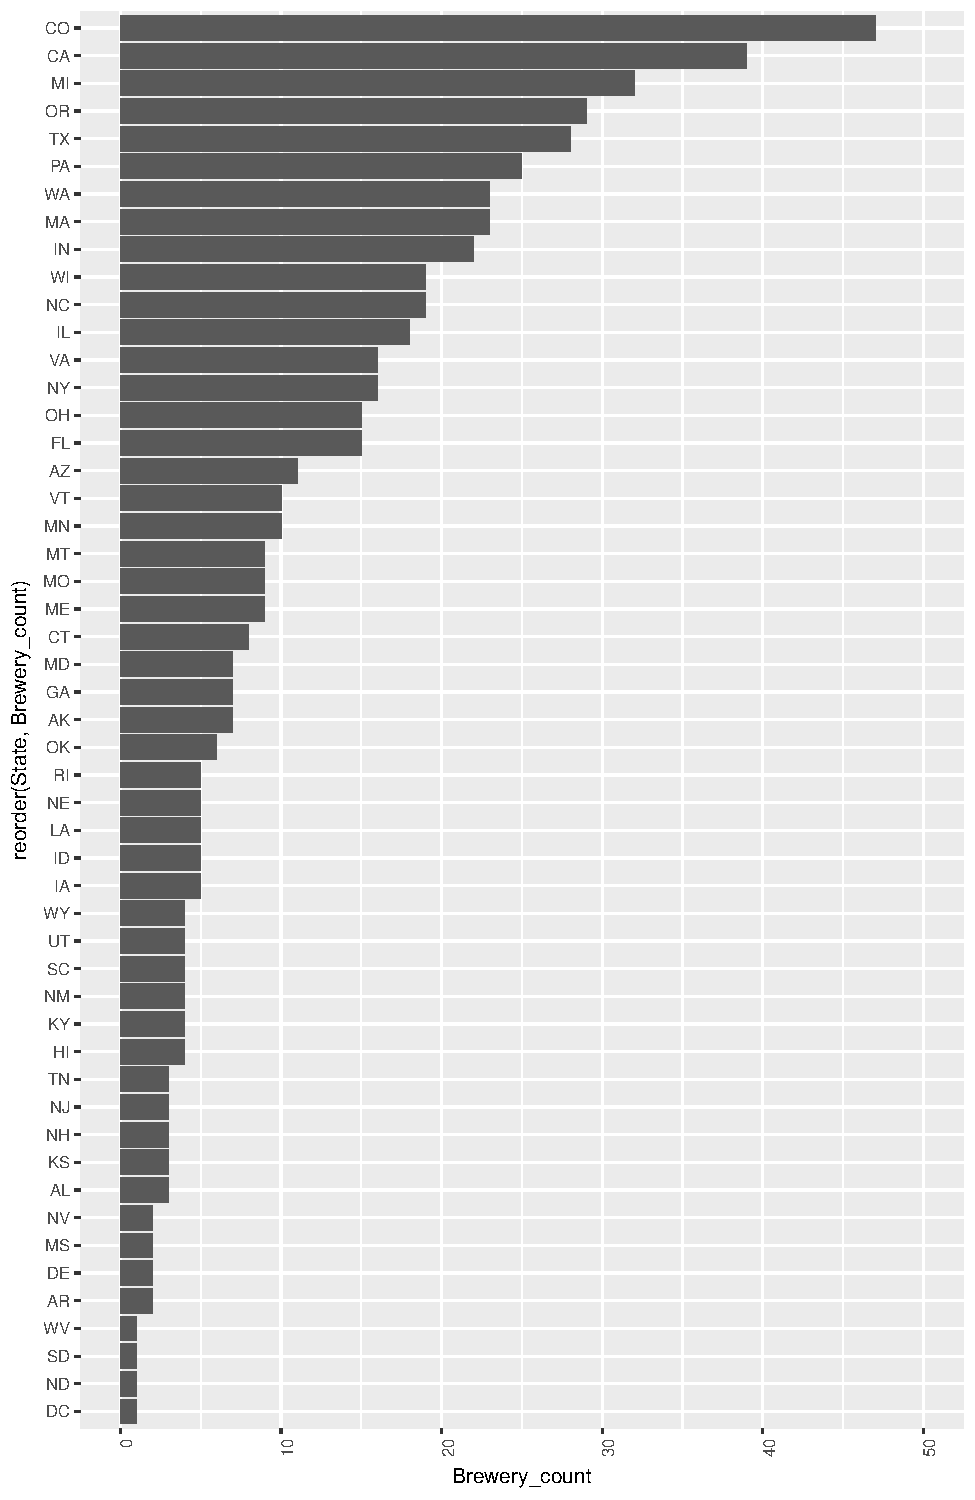
\includegraphics{stats_files/figure-latex/unnamed-chunk-8-1.pdf}

\begin{Shaded}
\begin{Highlighting}[]
  \CommentTok{#calulate line fit}
\NormalTok{  y <-}\StringTok{ }\KeywordTok{quantile}\NormalTok{((styles}\OperatorTok{$}\NormalTok{ABV }\OperatorTok\StringTok{ }\KeywordTok{na.omit}\NormalTok{()), }\KeywordTok{c}\NormalTok{(}\FloatTok{0.25}\NormalTok{, }\FloatTok{0.75}\NormalTok{))}
\NormalTok{  x <-}\StringTok{ }\KeywordTok{qnorm}\NormalTok{(}\KeywordTok{c}\NormalTok{(}\FloatTok{0.25}\NormalTok{, }\FloatTok{0.75}\NormalTok{))}
\NormalTok{  slope <-}\StringTok{ }\KeywordTok{diff}\NormalTok{(y)}\OperatorTok{/}\KeywordTok{diff}\NormalTok{(x)}
\NormalTok{  y_int <-}\StringTok{ }\NormalTok{y[}\DecValTok{1}\NormalTok{] }\OperatorTok{-}\StringTok{ }\NormalTok{slope }\OperatorTok{*}\StringTok{ }\NormalTok{x[}\DecValTok{1}\NormalTok{]  }
  
  \KeywordTok{ggplot}\NormalTok{(styles, }\KeywordTok{aes}\NormalTok{(}\DataTypeTok{sample =}\NormalTok{ styles}\OperatorTok{$}\NormalTok{ABV)) }\OperatorTok{+}\StringTok{ }
\StringTok{    }\KeywordTok{geom_qq}\NormalTok{(}\DataTypeTok{shape =} \DecValTok{16}\NormalTok{, }\DataTypeTok{size =} \DecValTok{2}\NormalTok{, }\DataTypeTok{alpha =} \FloatTok{0.5}\NormalTok{) }\OperatorTok{+}
\StringTok{    }\KeywordTok{geom_abline}\NormalTok{(}\DataTypeTok{slope =}\NormalTok{ slope, }\DataTypeTok{intercept =}\NormalTok{ y_int, }\DataTypeTok{colour =}\StringTok{'red'}\NormalTok{, }\DataTypeTok{size =} \DecValTok{1}\NormalTok{) }\OperatorTok{+}
\StringTok{    }\KeywordTok{ggtitle}\NormalTok{(}\StringTok{"QQplot of ABV"}\NormalTok{) }\OperatorTok{+}
\StringTok{    }\KeywordTok{theme_minimal}\NormalTok{()  }
\end{Highlighting}
\end{Shaded}

\includegraphics{stats_files/figure-latex/unnamed-chunk-8-2.pdf}

\section{Analysis using Spearman Rank-Order
Correlation}\label{analysis-using-spearman-rank-order-correlation}

\begin{verbatim}
+ More info on Spearman test: https://statistics.laerd.com/statistical-guides/spearmans-rank-order-correlation-statistical-guide.php
\end{verbatim}

\begin{itemize}
\tightlist
\item
  H\textsubscript{o}: \(\rho= 0\)
\item
  H\textsubscript{A}: \(\rho\neq 0\)
\end{itemize}

\begin{Shaded}
\begin{Highlighting}[]
\NormalTok{a=}\DecValTok{1}\OperatorTok{-}\NormalTok{.}\DecValTok{05}\OperatorTok{/}\DecValTok{2}


\NormalTok{ss}
\end{Highlighting}
\end{Shaded}

\begin{verbatim}
##                                    Style IBU   ABV Ounces
## 1016                 Munich Helles Lager  17 0.045     12
## 568              American Pale Ale (APA)  45 0.065     16
## 146                  American Blonde Ale  30 0.056     12
## 118                  American Blonde Ale  16 0.044     12
## 1143                             Witbier  16 0.050     16
## 341                         American IPA 104 0.060     16
## 707                       American Stout  26 0.057     16
## 826                     English Pale Ale  30 0.054     16
## 376                         American IPA  70 0.066     12
## 63              American Amber / Red Ale  25 0.059     16
## 958                              Kölsch  28 0.058     16
## 10                               Altbier  29 0.052     16
## 1102                        Scottish Ale  23 0.054     16
## 647                     American Pilsner  22 0.049     12
## 483              American Pale Ale (APA)  42 0.042     16
## 101                   American Black Ale  75 0.060     12
## 828                     English Pale Ale  17 0.051     12
## 87            American Amber / Red Lager  25 0.057     12
## 453                         American IPA  50 0.060     12
## 895                      German Pilsener  35 0.055     12
## 1010                 Munich Helles Lager  18 0.055     12
## 822         English India Pale Ale (IPA)  47 0.068     16
## 1027                             Old Ale  40 0.072     12
## 778                       Czech Pilsener  32 0.050     12
## 839  Extra Special / Strong Bitter (ESB)  32 0.056     12
## 419                         American IPA  30 0.045     12
## 293                         American IPA  85 0.068     12
## 179                   American Brown Ale  30 0.053     12
## 313                         American IPA 100 0.068     12
## 251       American Double / Imperial IPA  95 0.080     12
\end{verbatim}

\begin{Shaded}
\begin{Highlighting}[]
\NormalTok{m =}\StringTok{ "spearman"} \CommentTok{# ABV and IBU are both ordinal}

\CommentTok{#plot(styles$IBU, styles$ABV)}
\NormalTok{results <-}\StringTok{ }\KeywordTok{cor.test}\NormalTok{(styles}\OperatorTok{$}\NormalTok{IBU, styles}\OperatorTok{$}\NormalTok{ABV, }\DataTypeTok{method =}\NormalTok{ m, }\DataTypeTok{conf.level =}\NormalTok{ a)}
\end{Highlighting}
\end{Shaded}

\begin{verbatim}
## Warning in cor.test.default(styles$IBU, styles$ABV, method = m, conf.level
## = a): Cannot compute exact p-value with ties
\end{verbatim}

\begin{Shaded}
\begin{Highlighting}[]
\NormalTok{results}
\end{Highlighting}
\end{Shaded}

\begin{verbatim}
## 
##  Spearman's rank correlation rho
## 
## data:  styles$IBU and styles$ABV
## S = 89464000, p-value < 2.2e-16
## alternative hypothesis: true rho is not equal to 0
## sample estimates:
##       rho 
## 0.6386376
\end{verbatim}

\begin{Shaded}
\begin{Highlighting}[]
\NormalTok{r_sq <-}\StringTok{ }\NormalTok{results[[}\StringTok{"estimate"}\NormalTok{]][[}\StringTok{"rho"}\NormalTok{]]}\OperatorTok{^}\DecValTok{2}
\NormalTok{r_sq}
\end{Highlighting}
\end{Shaded}

\begin{verbatim}
## [1] 0.407858
\end{verbatim}

\begin{Shaded}
\begin{Highlighting}[]
\CommentTok{#qt(a, results[["parameter"]][["df"]])}



\NormalTok{results <-}\StringTok{ }\KeywordTok{cor.test}\NormalTok{(ss}\OperatorTok{$}\NormalTok{IBU, ss}\OperatorTok{$}\NormalTok{ABV, }\DataTypeTok{method =}\NormalTok{ m, }\DataTypeTok{conf.level =}\NormalTok{ a)}
\end{Highlighting}
\end{Shaded}

\begin{verbatim}
## Warning in cor.test.default(ss$IBU, ss$ABV, method = m, conf.level = a):
## Cannot compute exact p-value with ties
\end{verbatim}

\begin{Shaded}
\begin{Highlighting}[]
\NormalTok{results}
\end{Highlighting}
\end{Shaded}

\begin{verbatim}
## 
##  Spearman's rank correlation rho
## 
## data:  ss$IBU and ss$ABV
## S = 1385.3, p-value = 2.292e-05
## alternative hypothesis: true rho is not equal to 0
## sample estimates:
##       rho 
## 0.6918099
\end{verbatim}

\begin{Shaded}
\begin{Highlighting}[]
\NormalTok{r_sq <-}\StringTok{ }\NormalTok{results[[}\StringTok{"estimate"}\NormalTok{]][[}\StringTok{"rho"}\NormalTok{]]}\OperatorTok{^}\DecValTok{2}
\NormalTok{r_sq}
\end{Highlighting}
\end{Shaded}

\begin{verbatim}
## [1] 0.4786009
\end{verbatim}

\begin{Shaded}
\begin{Highlighting}[]
\CommentTok{#qt(a, results[["parameter"]][["df"]])}

\CommentTok{#plot(select(ss, IBU, ABV))}

\KeywordTok{print}\NormalTok{(}\StringTok{"There is strong evidence that the ABV and IBU are correlated (p-value > 0.001).  The IBU rating accounts for 40.7% of the variation in the ABV.  While IBU and ABV certainly have a correlation, that correlation is not very strong."}\NormalTok{) }\CommentTok{#TODO: calculate conf int}
\end{Highlighting}
\end{Shaded}

\begin{verbatim}
## [1] "There is strong evidence that the ABV and IBU are correlated (p-value > 0.001).  The IBU rating accounts for 40.7% of the variation in the ABV.  While IBU and ABV certainly have a correlation, that correlation is not very strong."
\end{verbatim}

\begin{Shaded}
\begin{Highlighting}[]
\CommentTok{#TODO: check number of ties}
\end{Highlighting}
\end{Shaded}

Alternative questions to ask: + Does the mean/median ABV of a brewery


\end{document}
